% ===================================================================
% CertiCut --- Physical Review A (Regular Article) version
% REVTeX 4.2, aps/pra, two-column reprint layout.
%
% The underlying science, theorems, and data are unchanged; the narrative
% is reordered so that the representation-sensitivity question and the
% quasiprobability resource semantics lead, with solver/backend and
% polyhedral engineering moved to the appendices.
%
% Section selection (submission form): A-2E Quantum Information Science.
% PhySH concepts (submission form, not typeset here):
%   Quantum information; Quantum computation; Quantum algorithms;
%   Quantum information processing; Optimization; Numerical methods.
% ===================================================================
\pdfminorversion=7  % allow inclusion of PDF v1.7 figures without warnings
\documentclass[
  aps,
  pra,
  reprint,
  amsmath,
  amssymb,
  longbibliography,
  nofootinbib
]{revtex4-2}

\usepackage{amsfonts}
\usepackage{amsthm}
\usepackage{booktabs}
\usepackage{graphicx}
\usepackage[hidelinks]{hyperref}

\graphicspath{{figures/}}

% Float-placement hygiene: allow more floats per page so the many appendix
% tables/figures do not get stuck, and soak up unbreakable inline math into
% the column gutter rather than overflowing the margin.
\setcounter{topnumber}{3}
\renewcommand{\topfraction}{0.92}
\setcounter{totalnumber}{4}
\renewcommand{\textfraction}{0.07}
\renewcommand{\floatpagefraction}{0.80}
\setcounter{dbltopnumber}{3}
\renewcommand{\dbltopfraction}{0.92}
\renewcommand{\dblfloatpagefraction}{0.80}
\emergencystretch=3em

% Theorem-like environments (plain style: bold header, italic body),
% independent counters so Theorem/Proposition/Corollary each number 1,2,...
\theoremstyle{plain}
\newtheorem{theorem}{Theorem}
\newtheorem{proposition}{Proposition}
\newtheorem{corollary}{Corollary}
% Suppress the QED box (kept from the source: it was mistaken for a
% missing-glyph square in the original build).
\renewcommand{\qedsymbol}{}

\newcommand{\CertiCut}{\textsc{CertiCut}}
\newcommand{\OPT}{\mathrm{OPT}}
\newcommand{\LB}{\mathrm{LB}}
\newcommand{\UB}{\mathrm{UB}}
\newcommand{\gap}{\Delta}

% Table fitting helpers (single- and full-width).
\newcommand{\tabfit}[1]{\resizebox{\columnwidth}{!}{#1}}
\newcommand{\tabfitscript}{\scriptsize}
\newcommand{\tabfitstar}[1]{\resizebox{\linewidth}{!}{#1}}

\begin{document}

\title{Representation-Sensitive Quantum Circuit Cutting with Quasiprobability Resource Bounds}

\author{Phung Trong Hung}
\email[Corresponding author: ]{phungtronghung0808@gmail.com}
\affiliation{Faculty of Information Technology, Ho Chi Minh City University of Technology (HUTECH), Ho Chi Minh City, Vietnam}

\author{Huong Bui}
\email{bd.huong@hutech.edu.vn}
\affiliation{Faculty of Information Technology, Ho Chi Minh City University of Technology (HUTECH), Ho Chi Minh City, Vietnam}

\date{}

% ===================================================================
% ABSTRACT
% ===================================================================
\begin{abstract}
Semantically equivalent quantum circuits can induce different gate-level quasiprobability costs after compilation, raising the question of whether a representation change can alter the optimal placement of circuit cuts. We formalize this effect for circuit cutting under a fixed independent quasiprobability-decomposition (QPD) model. We introduce a tie-safe cross-representation regret that compares optimal-placement sets rather than arbitrarily selected optima, derive a perturbation bound on this regret, and establish a sufficient stability condition together with positive-scaling invariance. Semantic-equivalence checks combined with a two-stage lexicographic optimization identify seven strict representation-induced placement reversals among 95 paired records. An exact quantum-phase-estimation instance exhibits a placement-regret factor of $729$, while six apparent quantum-Fourier-transform reversals obtained from single-optimum evaluation disappear under the tie-safe definition. Independently, algorithm-derived circuits show that minimizing the number of cuts can differ substantially from minimizing quasiprobability sampling overhead, with an exhaustively enumerated witness exceeding a factor of one million. For a fixed representation, we show that independent gate-level quasiprobability overhead reduces exactly to capacitated weighted graph partitioning in the logarithmic domain, so global optimization bounds translate directly into multiplicative resource bounds. A restricted joint-decomposition study further demonstrates that optimal placements can depend on the assumed resource model. These results expose circuit representation as a relevant degree of freedom in resource-aware circuit cutting and provide quantitative conditions under which cut-placement decisions remain stable. We package the analysis and its frozen evidence as an auditable framework, \CertiCut{}.
\end{abstract}

\maketitle

% ===================================================================
% I. INTRODUCTION
% ===================================================================
\section{Introduction}
\label{sec:intro}

Near-term quantum processors remain limited in qubit count, fidelity, and connectivity~\cite{preskill2018}. Circuit cutting mitigates the width constraint by decomposing a circuit into smaller, independently executable fragments and recovering the target observable through classical post-processing~\cite{peng2020,bravyi2016,tang2021}. This decomposition is not free: every severed two-qubit interaction contributes a gate-dependent quasiprobability sampling factor, and these factors multiply across cuts. Minimizing the number of cuts therefore need not minimize the resulting sampling overhead.

A quantum circuit does not possess a unique gate-level representation. Compilation, basis translation, and native-gate decomposition each produce semantically equivalent circuits---identical unitaries up to a global phase---whose two-qubit interaction structure, and hence whose gate-level quasiprobability costs, generally differ. This exposes a question that is invisible at the level of cut counting: holding the logical circuit and its feasible partition space fixed, can a semantically equivalent \emph{representation} change \emph{which} placement of cuts is optimal, and by how much does a placement that is optimal for one representation inflate the sampling overhead when it is transported to another? A naive comparison that solves each representation once and cross-evaluates the two selected optima can report such an effect spuriously whenever the optimizer chooses arbitrarily among tied optima. Distinguishing a genuine representation-induced reversal from a tie-breaking artifact therefore requires comparing optimal-placement \emph{sets}, not individual optima.

A second, orthogonal question concerns the guarantee attached to any computed placement. Automatic cutting workflows commonly report a partition together with a solver-specific status. Although mixed-integer programming (MIP) exposes primal and dual bounds, their implication for the physical sampling overhead is not explicit in the solver output, and an additive objective gap can represent orders of magnitude of multiplicative sampling cost. Working in the log-overhead domain makes the connection exact: a valid global optimization gap immediately yields a worst-case multiplicative overhead ratio, so a practitioner obtains not merely a partition but a bound on its distance from the modeled optimum.

We address both questions within a single framework, which we call \CertiCut{}, built on a fixed independent quasiprobability-decomposition (QPD) cost model. The formulation targets logical interaction graphs, supports arbitrary declared fragment counts and per-fragment lower/upper capacities, and uses independent gate-level QPD costs from Qiskit Addon Cutting~0.10.0~\cite{qiskitcutting}, which supports SparsePauliOp-oriented reconstruction workflows compatible with the partitions we certify. The resource-bound framework and the representation study answer one linked question: valid bounds identify which placements remain resource-competitive, while tie-safe comparison determines whether a representation change can alter that decision. In exact arithmetic, global bounds at a safe stopping boundary imply a multiplicative overhead factor $F=\exp(\UB-\LB)$. Production MIP bounds, factors, closures, and lexicographic outcomes are floating-point solver-tolerance quantities rather than exact-arithmetic certificates; we mark this distinction explicitly throughout and reserve the word \emph{certificate} in its strong sense for a small CX-only tier verified by exact interval arithmetic.

\begin{figure*}[tp]
  \centering
  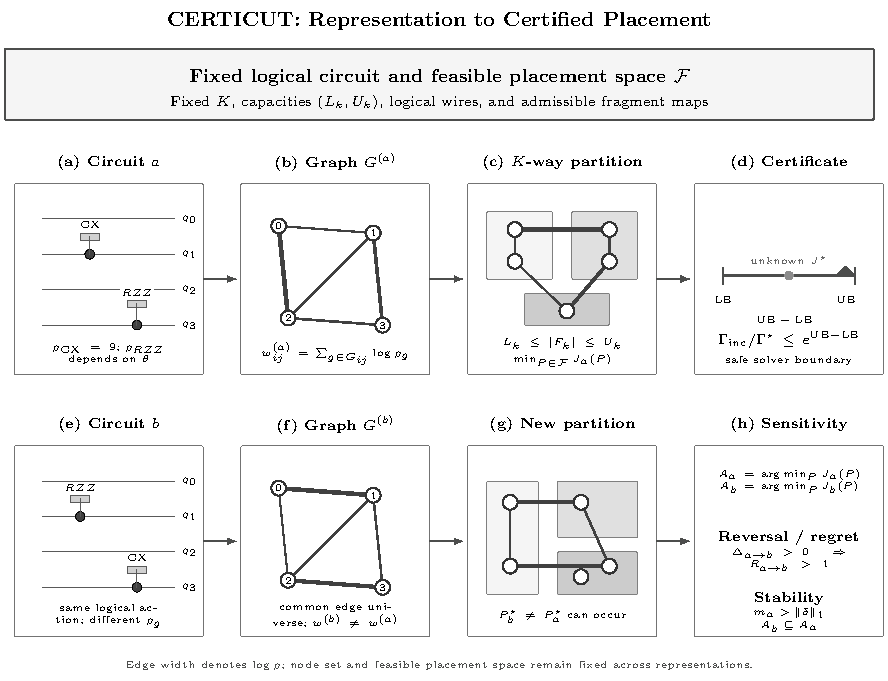
\includegraphics[width=0.95\textwidth]{figures/fig_certicut_architecture.pdf}
  \caption{\CertiCut{} conceptual model. A fixed logical circuit and capacitated feasible placement space induce representation-specific independent-QPD interaction weights. Fixed-representation optimization converts any valid global MIP gap into the multiplicative overhead bound $\Gamma_{\mathrm{inc}}/\Gamma^*\leq\exp(\UB-\LB)$. Tie-safe comparison of the resulting optimal-placement sets then quantifies representation-induced regret or establishes placement stability.}
  \label{fig:architecture}
\end{figure*}

\CertiCut{} contributes three linked circuit-cutting results: (i)~a representation-placement theory built on tie-safe regret, margin stability, and positive-scaling invariance; (ii)~resource-semantic bounds $\Gamma_{\mathrm{inc}}/\Gamma^*\le\exp(\UB-\LB)$; and (iii)~an exact capacitated $K$-way independent-QPD reduction to a log-domain graph MIP. These results belong together because the MIP instantiates a set-level decision problem, while global bounds put representation-specific decisions on a common resource scale without conflating a solver-selected tie with a true reversal. Weighted graph partitioning, branch and bound, capacities, cardinality identities, and metric inequalities are established machinery~\cite{deza1997,lawler1966,kaibel2008}; our claim is the representation-placement analysis and its resource semantics, not a new generic partitioning algorithm.

This work therefore makes three primary contributions:
\begin{enumerate}
  \item \emph{Representation-sensitive placement theory and evidence.} We define tie-safe cross-representation regret $R_{a\to b}$, prove perturbation stability and positive-scaling invariance, and confirm placement reversals on quantum phase estimation (QPE, the operationally relevant witness, $R=729$) and Grover circuits with a two-stage lexicographic MIP across $\tau_{\mathrm{opt}}\in\{10^{-8},10^{-9},10^{-10}\}$, while ruling out single-solve false positives on the quantum Fourier transform (QFT). These medium-tier reversals are robust across the $\tau_{\mathrm{opt}}$ sweep rather than independently certified in exact arithmetic; a separate CX-only tier is certified by verified interval enumeration.
  \item \emph{Interpretable resource bounds.} In exact arithmetic, any valid global pair $(\UB,\LB)$ guarantees $\Gamma_{\mathrm{inc}}/\Gamma^*\leq\exp(\UB-\LB)$. Implementation outputs are explicitly solver-tolerance quantities, not exact-arithmetic certificates, and are usable with mature MIP solvers.
  \item \emph{Exact capacitated $K$-way independent-QPD reduction.} For arbitrary $K\geq2$, lower/upper fragment capacities, a fixed representation, and independent per-gate QPD, the assignment/locality MIP exactly optimizes the modeled log-overhead, and exponentiation recovers the multiplicative sampling overhead.
\end{enumerate}
The central novelty is not that semantically equivalent representations carry different gate counts or absolute QPD costs, but that they can induce different \emph{optimal fragment-placement sets}, and that naive single-optimum cross-evaluation can falsely report such an effect whenever optimizer-selected ties exist.

This positioning is deliberately distinct from recent circuit-cutting optimizers. Brandhofer \emph{et al.}~\cite{brandhofer2024} minimize sampling overhead over a richer space of mixed gate and wire cuts; Nakamura \emph{et al.}~\cite{nakamura2025} improve sampling bounds and scalable partitioning beyond bipartitions; and Fr{\"o}hler \emph{et al.}~\cite{frohler2026} give a scalable heuristic framework spanning gate, wire, and joint gate-group cuts. All three seek \emph{cheaper cuts} for a fixed circuit. \CertiCut{} asks an orthogonal question: holding the logical circuit and its feasible placement space fixed, can a semantically equivalent \emph{representation} change which placement is optimal, and can that decision be certified against optimizer-selected ties? Our contribution is thus optimal-set representation sensitivity, tie-safe set-level comparison, and solver-tolerance resource semantics---not a faster or lower-overhead partitioner, and not a new graph-partitioning algorithm. We make no speed claim on the shared independent gate-QPD scale; indeed, an off-the-shelf MIP solver outperforms our specialized reference search in the backend comparison of Appendix~\ref{app:backend}.

\subsection{Why solve a declared, non-optimal model exactly}
\label{sec:why-exact}

Independent per-gate QPD is not the tightest available cut-cost model: joint and communication-assisted decompositions can be strictly cheaper, and our own restricted-joint witness (Sec.~\ref{sec:results-joint}) shows the independent optimum a factor $1.90\times$ worse when re-evaluated under a parallel-joint semantics. We nonetheless optimize this model \emph{exactly}, rather than approximately optimizing a stronger one, for three deliberate reasons. First, it is the model production tooling actually deploys: Qiskit Addon Cutting~0.10.0~\cite{qiskitcutting} generates and recombines subexperiments under exactly this independent gate-QPD accounting, so an exact placement for this model is directly usable in that pipeline today, whereas an approximate placement for a richer model is not yet supported end to end by that stack. Second, exactness is what makes the resource claim auditable: a valid global optimization gap for the declared model translates, with no further modeling assumption, into a certified worst-case multiplicative overhead (Theorem~\ref{thm:gap}), so a practitioner obtains not merely a partition but a bound on its distance from the model optimum. Third, and most importantly, the representation-sensitivity effect we isolate is orthogonal to absolute model strength---it concerns \emph{which} placement is optimal, not its absolute cost---so it can only be exhibited and certified against an exactly solved reference. The same set-level analysis applies whenever a model induces representation-dependent interaction weights; heterogeneity is necessary but, as our results show, not sufficient to force a reversal. Approximately optimizing a stronger model would confound representation effects with optimization error. Solving the declared model exactly thus trades absolute cost optimality---which we quantify and bound rather than conceal---for decision-level rigor.

\subsection{Scope of the resource-model and verified-arithmetic studies}
\label{sec:scope-preview}

Two further studies delimit the scope of the resource claims and are reported in full in the results and appendices. First, independent QPD is a declared cut-cost model, not an assertion that stronger joint decompositions preserve placements. Section~\ref{sec:results-joint} exhibits a controlled six-qubit witness under a theorem-guarded library of pairwise-disjoint same-layer gate groups for which the independent optimum is $1.90496\times$ worse under a restricted parallel-joint semantics, and it tests algorithm-derived native-QPD circuits under the same library. This is a scope stress test, not a claim that \CertiCut{} optimizes general joint QPD. Second, to ground the word ``certificate'' in at least one rigorously verified setting, Appendix~\ref{app:verified} certifies a small CX-only tier using exact interval arithmetic with 80-decimal directed intervals for $\log 9$, rather than solver bounds. Every medium- and large-tier factor reported here is instead an explicitly solver-tolerance quantity, and the two are never conflated.

The remainder is organized as follows. Section~\ref{sec:model} fixes the independent-QPD cost model and the log-domain interaction graph and defines representation changes. Section~\ref{sec:rep} develops the representation-sensitive placement theory: tie-safe regret, a perturbation bound, a stability theorem, and positive-scaling invariance. Section~\ref{sec:opt} gives the exact capacitated $K$-way formulation and the gap-to-overhead resource semantics. Section~\ref{sec:results} reports the numerical evidence---representation reversals, count-versus-QPD reversals, capacitated scaling, resource-model sensitivity, and finite-shot scope. Section~\ref{sec:related} places the work among related cut-placement research, and Secs.~\ref{sec:discussion} and~\ref{sec:conclusion} discuss limitations and conclude. Appendices~\ref{app:backend}--\ref{app:verified} provide the optimization backends and reference implementation, the polyhedral ablations, and the verified interval tier. Throughout, we separate circuit-cutting model semantics from optimization-backend performance.

% ===================================================================
% II. MODEL
% ===================================================================
\section{Circuit cutting and representation-dependent quasiprobability costs}
\label{sec:model}

\subsection{Independent-QPD circuit cutting}

Gate cutting replaces selected two-qubit channels by quasiprobability decompositions (QPDs) over fragment-local channels~\cite{peng2020,mitarai2021}. For a cuttable channel $\mathcal{U}_g=\sum_i a_{g,i}\mathcal{E}_{g,i}$, the corresponding independent sampling overhead is
\begin{equation}
  \rho_g = \left(\sum_i |a_{g,i}|\right)^{\!2}.
  \label{eq:gate-overhead}
\end{equation}
For a partition $P$ with crossed-gate set $S(P)$, independent sampling across gates gives
\begin{equation}
  \Gamma(P) = \prod_{g \in S(P)} \rho_g, \qquad
  J(P) = \log \Gamma(P) = \sum_{g \in S(P)} \log \rho_g.
  \label{eq:objective}
\end{equation}
This objective matches the independent gate-level model in Qiskit Addon Cutting~0.10.0~\cite{qiskitcutting}; it is not a model of joint decompositions, finite-shot variance, or hardware noise. Because the QPD coefficient one-norm is at least one, $\rho_g\geq1$ and all log weights are nonnegative. We validated the gate costs against the Qiskit QPD registry: $\rho_{\mathrm{CX}}=\rho_{\mathrm{CZ}}=9$, $\rho_{\mathrm{iSWAP}}=\rho_{\mathrm{DCX}}=49$, $\rho_{\mathrm{CS}}=3+2\sqrt{2}\approx5.828$, and $\rho_{RZZ(\theta)}=(1+2|\sin\theta|)^2$ for numerically bound rotations.

\subsection{Log-domain interaction graph}

Let $V=\{0,\ldots,n{-}1\}$ be the circuit qubits, and let $G_{ij}$ contain the two-qubit gate occurrences acting on pair $(i,j)$. We assign the nonnegative interaction weight
\begin{equation}
  w_{ij} = \sum_{g \in G_{ij}} \log \rho_g.
  \label{eq:weight}
\end{equation}
For any fragment map $f:V\rightarrow\{1,\ldots,K\}$, the objective becomes
\begin{equation}
  J(P) = \sum_{i < j} w_{ij} \cdot \mathbb{I}(f(i)\neq f(j)).
  \label{eq:graph-objective}
\end{equation}
The binary bisection identity $\mathbb{I}(f(i)\neq f(j))=|z_i-z_j|$ is recovered when $K=2$.

\begin{proposition}[Objective equivalence]\label{prop:obj-equiv}
Under independent gate-level QPD, minimizing~\eqref{eq:objective} is equivalent to minimizing~\eqref{eq:graph-objective}.
\end{proposition}
\begin{proof}
Every $g\in G_{ij}$ is cut exactly when $f(i)\neq f(j)$. Regrouping the gate-level sum by qubit pair yields~\eqref{eq:graph-objective}.
\end{proof}

\subsection{Representation changes and the common edge universe}
\label{sec:rep-changes}

A fixed logical circuit admits many semantically equivalent gate-level representations: transpilation to a target basis, native-gate decomposition, and optimization passes each preserve the implemented unitary up to a global phase while altering the two-qubit interaction multigraph, and hence the weights~\eqref{eq:weight}. Let $a$ and $b$ be two semantically equivalent representations of the same logical circuit on the same logical wire set $V$, with interaction edge sets $E_a$ and $E_b$. We define the common edge universe $E=E_a\cup E_b$ and zero-pad the log-weights, $w^{(a)}_e=0$ for $e\notin E_a$ and $w^{(b)}_e=0$ for $e\notin E_b$, so that both representations are compared over a single feasible partition space. Because the two representations implement the same unitary, any cut placement is physically admissible for both; what changes is the interaction weight carried across the cut. Section~\ref{sec:rep} makes precise the sense in which a change from $a$ to $b$ can move the optimal placement.

% ===================================================================
% III. REPRESENTATION THEORY
% ===================================================================
\section{Representation-sensitive optimal cut placement}
\label{sec:rep}

\subsection{Tie-safe placement regret}
\label{sec:tie-safe}

Consider the fixed logical qubit set $V=\{0,\ldots,n{-}1\}$ evaluated over a common feasible partition space $\mathcal{F}$ defined by a declared fragment count $K$ and capacity bounds. For any partition $P\in\mathcal{F}$, the log objectives of the two representations are $J_a(P)=(w^{(a)})^\top z(P)$ and $J_b(P)=(w^{(b)})^\top z(P)$, where $z(P)\in\{0,1\}^{|E|}$ is the cut-indicator vector over the common edge universe $E$ of Sec.~\ref{sec:rep-changes}. Let $\mathcal{A}_a=\arg\min_{P\in\mathcal{F}}J_a(P)$ and $J_b^*=\min_{P\in\mathcal{F}}J_b(P)$. The \emph{tie-safe cross-representation regret} and the corresponding sampling overhead factor are
\begin{equation}
  \Delta_{a\to b} = \min_{P \in \mathcal{A}_a} J_b(P) - J_b^*, \qquad R_{a\to b} = \exp(\Delta_{a\to b}).
  \label{eq:regret}
\end{equation}
The minimum over $\mathcal{A}_a$ makes the metric tie-safe and conservative: it reports positive regret only when \emph{every} $a$-optimal placement is suboptimal under $b$; it is not a worst-case arbitrary-tie-breaking metric. When $R_{a\to b}=1$, at least one optimal partition under representation $a$ remains optimal under $b$ ($\mathcal{A}_a\cap\mathcal{A}_b\neq\varnothing$). When $R_{a\to b}>1$, every optimal partition under $a$ is strictly suboptimal under $b$. In general $R_{a\to b}\neq R_{b\to a}$.

\subsection{Representation-regret bound}

The following perturbation statements are exact model-level results; the medium-tier numerical evaluations of Sec.~\ref{sec:results} are solver-tolerance quantities. Let $\delta=w^{(b)}-w^{(a)}\in\mathbb{R}^{|E|}$ be the interaction-weight perturbation vector over the edge universe $E$.

\begin{proposition}[Representation-regret bound]\label{prop:regret-bound}
For any common feasible partition space $\mathcal{F}$, $0\le\Delta_{a\to b}\le\|\delta\|_1$, and $R_{a\to b}\le\exp(\|\delta\|_1)$.
\end{proposition}
\begin{proof}
Let $P_a\in\arg\min_{P\in\mathcal{A}_a}J_b(P)$ and $P_b\in\mathcal{A}_b$. Then $J_b(P_a)-J_b(P_b)=[J_a(P_a)-J_a(P_b)]+\delta^\top[z(P_a)-z(P_b)]$. Because $P_a$ is $J_a$-optimal, $J_a(P_a)-J_a(P_b)\le0$. Since $[z(P_a)-z(P_b)]_e\in\{-1,0,1\}$, we obtain $\Delta_{a\to b}\le\delta^\top[z(P_a)-z(P_b)]\le\|\delta\|_1$.
\end{proof}

\subsection{Stability theorem and scaling invariance}

Let $m_a=\min_{P\in\mathcal{F}\setminus\mathcal{A}_a}[J_a(P)-J_a^*]$ denote the optimality margin of representation $a$, with the convention $m_a=+\infty$ if $\mathcal{F}\setminus\mathcal{A}_a=\emptyset$.

\begin{theorem}[Representation stability]\label{thm:stability}
If $m_a>\|\delta\|_1$, then $\mathcal{A}_b\subseteq\mathcal{A}_a$, and consequently $R_{a\to b}=1$.
\end{theorem}
\begin{proof}
For any $P\in\mathcal{A}_a$ and $Q\in\mathcal{F}\setminus\mathcal{A}_a$, $J_a(Q)-J_a(P)\ge m_a$. The perturbation changes the objective difference by at most $|\delta^\top[z(Q)-z(P)]|\le\|\delta\|_1$. If $m_a>\|\delta\|_1$, then $J_b(Q)-J_b(P)\ge m_a-\|\delta\|_1>0$, so no non-optimal partition $Q\notin\mathcal{A}_a$ can achieve a smaller or equal $J_b$ objective than $P$. Thus $\mathcal{A}_b\subseteq\mathcal{A}_a$, guaranteeing $R_{a\to b}=1$.
\end{proof}

Defining $\kappa_{a\to b}=\|\delta\|_1/m_a$, the condition $\kappa_{a\to b}<1$ is a sufficient condition for placement stability.

\begin{corollary}[Positive-scaling invariance]\label{cor:scaling}
If $w^{(b)}=c\,w^{(a)}$ for $c>0$, then $\mathcal{A}_a=\mathcal{A}_b$ and $R_{a\to b}=R_{b\to a}=1$.
\end{corollary}
\begin{proof}
For any $P\in\mathcal{F}$, $J_b(P)=c\,J_a(P)$. Since $c>0$, the scalar multiplier preserves the exact partition-objective ordering, so $\arg\min J_a=\arg\min J_b$ and $R_{a\to b}=R_{b\to a}=1$.
\end{proof}

\subsection{Tie-safe evaluation protocol, orbitopes, and tolerances}
\label{sec:tie-safe-protocol}

Label-permutation symmetry is endemic to assignment formulations of partitioning. SCIP~10.0.2 can impose partitioning-orbitope constraints that keep only lexicographically maximal fragment-label matrices under the symmetric group acting on columns~\cite{kaibel2008}. These constraints address fragment-label symmetry: renaming fragments permutes assignment columns but leaves every cut-indicator vector $z(P)$ unchanged. Orbitopes remove redundant fragment-label permutations, but they cannot eliminate distinct primary-optimal partitions having different cut-indicator vectors. Consequently, a single MIP solve that returns one $a$-optimum and evaluates it under $b$ can report a spurious positive $\Delta_{a\to b}$ whenever another $a$-optimum would have been jointly optimal under $b$. Symmetry breaking therefore does not replace the second lexicographic optimization required to evaluate tie-safe regret. Stage~1 computes $J_a^*$ and $J_b^*$; Stage~2 minimizes $J_b(P)$ subject to $J_a(P)\le J_a^*+\tau_{\mathrm{opt}}$, and the reverse direction yields $\Delta_{b\to a}$. Thus Stage~2 is not merely a numerical tie-break: up to the declared lexicographic tolerance $\tau_{\mathrm{opt}}$, it implements the set-level optimization underlying the definition of $\Delta_{a\to b}$.

The lexicographic tolerance $\tau_{\mathrm{opt}}$ is not an arbitrary soft margin. It must sit strictly above the solver's internal numerical feasibility/integrality tolerances while remaining far below any relevant modeled log-overhead separation on the studied instances. Writing $\varepsilon_{\mathrm{SCIP}}$ for SCIP's effective feasibility/integrality tolerance (in SCIP both the constraint-feasibility and integrality checks are governed by \texttt{numerics/feastol}), we require
\begin{equation}
  \varepsilon_{\mathrm{SCIP}}
  \;\ll\;
  \tau_{\mathrm{opt}}
  \;\ll\;
  \min\bigl\{m_a,\,m_b,\,1\bigr\}
  \label{eq:tau-hierarchy}
\end{equation}
whenever the relevant optimality margins are finite. The left-hand separation is enforced directly by the pinned \texttt{numerics/feastol} value. The right-hand separation is not independently certified on the medium tier; robustness there is assessed by the three-value $\tau_{\mathrm{opt}}$ sweep. For the representation-regret rerun, every Stage-1 and Stage-2 SCIP model explicitly pins \texttt{numerics/feastol}$=10^{-12}$, so the sweep $\tau_{\mathrm{opt}}\in\{10^{-8},10^{-9},10^{-10}\}$ satisfies the left-hand separation. The sweep checks numerical robustness of the tolerance-defined lexicographic formulation; it does not by itself establish conclusions for an exact real-arithmetic decision problem. Exhaustive enumeration is used for $n\le10$; the lexicographic MIP covers $n\in\{12,14,16\}$ under PySCIPOpt~6.2.1 and Qiskit~2.5.1 / Addon Cutting~0.10.0.

% ===================================================================
% IV. OPTIMIZATION AND BOUNDS
% ===================================================================
\section{Capacitated formulation and resource bounds}
\label{sec:opt}

\subsection{Capacitated $K$-way partition problem}

Let $K\geq2$ be the declared fragment count. Binary assignment $a_{ik}=1$ denotes that qubit $i$ belongs to fragment $k$, with capacities $L_k\leq\sum_i a_{ik}\leq U_k$. For each aggregated interaction edge $e=(i,j)$, locality variable $y_{ek}=1$ denotes that both endpoints occupy fragment $k$, while $z_e=1$ denotes a crossed interaction. The exact independent-QPD MIP is
\begin{equation}
\begin{aligned}
\min\quad & \sum_{e\in E} w_e z_e\\
\text{s.t.}\quad & \sum_{k=1}^{K} a_{ik}=1 && \forall i,\\
& L_k\leq\sum_i a_{ik}\leq U_k && \forall k,\\
& y_{ek}\leq a_{ik},\quad y_{ek}\leq a_{jk} && \forall e=(i,j),k,\\
& y_{ek}\geq a_{ik}+a_{jk}-1 && \forall e=(i,j),k,\\
& z_e+\sum_{k=1}^{K}y_{ek}=1 && \forall e,\\
& a_{ik},y_{ek},z_e\in\{0,1\}.&
\end{aligned}
\label{eq:kway}
\end{equation}
The three inequalities are the exact binary AND hull. Since each endpoint has exactly one assignment, exactly one $y_{ek}$ is one iff both endpoints share a fragment; otherwise all locality variables are zero and $z_e=1$. Thus~\eqref{eq:kway} exactly optimizes~\eqref{eq:graph-objective} for arbitrary feasible capacities.

\begin{proposition}[Objective equivalence for capacitated $K$-way partitioning]\label{prop:kway-equiv}
For any $K\geq2$ and feasible capacities, the objective of~\eqref{eq:kway} equals the independent gate-level log overhead~\eqref{eq:objective}.
\end{proposition}
\begin{proof}
The assignment/locality constraints set $z_e=1$ exactly when the endpoints of aggregate edge $e$ are in different fragments. Equation~\eqref{eq:weight} sums the log overhead of every gate occurrence in $G_e$. Regrouping~\eqref{eq:objective} by edge yields $\sum_e w_ez_e$.
\end{proof}

Problem~\eqref{eq:kway} is NP-hard because exact-balanced weighted bisection is its $K=2$ special case.

\subsection{Fixed-capacity cardinality identity}

If fragment sizes are fixed exactly as $|F_k|=n_k$, every feasible partition crosses
\begin{equation}
  \sum_{i<j}\mathbb{I}(f(i)\neq f(j))
  = \binom{n}{2}-\sum_{k=1}^{K}\binom{n_k}{2}
  = \frac12\left(n^2-\sum_{k=1}^{K}n_k^2\right)
  \label{eq:kway-cardinality}
\end{equation}
complete-graph pairs. This is a structural identity, not a constraint for lower/upper-only capacities. Exact-balanced bisection is the special case $K=2$, $n_1=n_2=n/2$, yielding $n^2/4$. This identity, and the polyhedral strengthenings it enables, underlie the $K=2$ reference implementation and the negative polyhedral ablation reported in Appendix~\ref{app:poly}.

\subsection{Gap-to-overhead resource bounds}

\begin{theorem}[Gap-to-overhead translation, exact arithmetic]\label{thm:gap}
For any $K\geq2$, feasible capacity bounds, and optimization backend, if $\LB\leq\OPT\leq\UB$, where $\UB=J(P_{\mathrm{inc}})$ for a feasible incumbent of~\eqref{eq:kway}, then
\begin{equation}
  \frac{\Gamma(P_{\mathrm{inc}})}{\Gamma^*}
  = \exp(\UB-\OPT) \leq \exp(\UB-\LB).
  \label{eq:gap-translation}
\end{equation}
\end{theorem}
\begin{proof}
Equation~\eqref{eq:objective} gives $\Gamma(P)=\exp(J(P))$. Since $\OPT\geq\LB$, exponentiation yields~\eqref{eq:gap-translation}.
\end{proof}

This result depends on the specified independent-QPD objective and on valid global bounds, not on how a backend obtains them. Proposition~\ref{prop:safe-boundary} (Appendix~\ref{app:backend}) establishes the required bound premise for the $K=2$ \CertiCut{} reference search in exact arithmetic; mature MIP solvers supply the same premise through their own dual bounds.

\subsection{Numerical-bound semantics}
\label{sec:num-semantics}

Theorem~\ref{thm:gap} is an exact-arithmetic statement: in ideal mathematics, valid global bounds yield \emph{anytime resource bounds} $\Gamma_{\mathrm{inc}}/\Gamma^*\le\exp(\UB-\LB)$. In practice, every experimental bound, factor, closure, and MIP-derived regret reported here uses floating-point HiGHS or SCIP output and is a \emph{solver-tolerance bound}, not an independently verified numerical proof. The main \CertiCut{} protocol pairs SCIP's documented \texttt{numerics/feastol}$=10^{-6}$ with an externally declared $10^{-9}$ objective-gap closure criterion, while the reference LP solves use a separately stated $10^{-9}$ LP numerical tolerance and the representation-regret rerun pins \texttt{numerics/feastol}$=10^{-12}$; these tolerances are kept distinct throughout so that no reader infers a single shared value. This explicit distinction removes any real-number-theoretic ambiguity: the reported bounds are valid relative to solver-declared tolerances, not as exact-arithmetic guarantees. A formal numerical bound would additionally require verified conservative lower-bound recovery with outward rounding or rational/interval verification. We reserve the word \emph{certificate} in its strong sense only for the CX-only interval tier of Appendix~\ref{app:verified}.

% ===================================================================
% V. RESULTS
% ===================================================================
\section{Numerical results}
\label{sec:results}

\subsection{Computational protocol}
\label{sec:protocol}

All experiments use a frozen software and hardware protocol: Python~3.11.9, Qiskit~2.5.1, Qiskit Addon Cutting~0.10.0, Qiskit Aer~0.17.2, SciPy~1.17.1~\cite{scipy}, KaHIP~3.25~\cite{kahip}, MQT~Bench~2.2.2~\cite{mqtbench}, PySCIPOpt~6.2.1, and SCIP~10.0.2~\cite{scip}, on Windows~11 (build~26200) with an Intel Core i5-14400 (10 physical cores, 16 logical processors) and 31.69~GB RAM. Revision runners pin OpenMP, OpenBLAS, and MKL to one thread before numerical imports. The primary evidence corpus was frozen on August~11--12, 2026, and the predeclared validation and stress-test tracks on August~13--14, 2026; each track is versioned separately with its own raw records and SHA-256 manifest. As stated in Sec.~\ref{sec:num-semantics}, every reported optimization bound, factor, closure, and lexicographic outcome is a floating-point solver-tolerance quantity except for the interval tier of Appendix~\ref{app:verified}. The benchmark matrices are fixed designs rather than IID samples, so reported proportions are descriptive rather than population-prevalence estimates. Complete versions, seeds, solver tolerances, and integrity manifests are listed in Appendix~\ref{app:verified} and in the Data Availability statement. In accordance with APS policy on the use of AI tools, we disclose that generative AI assistants (large language models) were used to help implement and debug the experiment and analysis code; all code was reviewed, executed, and validated by the authors against the exhaustive-enumeration and interval oracles described below, and all scientific claims, derivations, and conclusions are the authors' own.

\subsection{Representation construction and semantic checks}
\label{sec:rep-construction}

Each paired record is derived from one frozen logical source circuit, identified by a shared source fingerprint. Both constructions retain exactly the same logical wire set $V$ and introduce no ancilla wires. The CX-normalized representation uses Qiskit's transpiler with basis $\{\texttt{rz},\texttt{sx},\texttt{x},\texttt{cx}\}$, optimization level~1, and fixed seed~0; the native-QPD representation recursively decomposes while retaining supported native two-qubit gates. Both use \texttt{coupling\_map=None}, so routing does not change logical qubits or inject topology-dependent operations. For every successfully ingested small-tier record ($n\le10$), the artifact materializes both Qiskit \texttt{Operator} matrices and checks $U_a^\dagger U_b=e^{i\phi}I$ to tolerance $10^{-6}$; the observed maximum deviation is $3.23\times10^{-14}$. For the nine headline pairs, QPE, QAOA, and QFT at $n\in\{12,14\}$ are independently verified up to global phase using dense miter checks where tractable and bounded QCEC~\cite{peham2022zx_equivalence} otherwise, while Grover at $n\in\{12,14,16\}$ uses a declared compositional proof (common source fingerprint and wire order, \texttt{coupling\_map=None}, no dynamic/classical operations or inserted routing, recursive native-definition expansion, and a semantics-preserving CX-basis transpilation). All nine pairs pass. This does not reinterpret practical QCEC timeouts as proofs.

\subsection{Representation-induced placement reversals}
\label{sec:results-reversals}

A representation change affects not only absolute independent-QPD resource costs but can alter the optimal partition placement itself. Table~\ref{tab:e12_regret} summarizes the tie-safe cross-representation regret across 95 paired records. Two findings form the headline: an operationally relevant QPE placement reversal of factor $R=729$, and (Sec.~\ref{sec:results-qft}) the elimination of six apparent QFT reversals that a naive single-solve evaluation reports as real. Grover enters only as a non-physical mathematical stress test of the metric.

Overall, $7/95$ ($7.4\%$) records exhibit a strict tie-safe placement reversal, on QPE and Grover circuits. The operationally relevant headline witness is exact QPE at $n=14$, $K=2$, where $\Delta_{\mathrm{native}\to\mathrm{CX}}=6.5917$ ($\log_{10}R=2.86$, $R=729.0$): adopting the placement optimal for one representation while evaluating it under the other inflates the modeled sampling overhead by three orders of magnitude. Because $R$ is a ratio of two placement costs, it quantifies relative placement regret rather than certifying that either absolute overhead is small. The Grover reversals occupy the opposite regime and are retained only as a mathematical stress test of the tie-safe machinery at extreme perturbation scale. Their optimal log-overheads are themselves non-physical: the largest, at $n=16$, $K=3$, has $\Delta_{\mathrm{CX}\to\mathrm{native}}=9984.19$ ($\log_{10}R=4336.1$), with CX-normalized and native representations of $234{,}300$ and $395{,}044$ two-qubit gate occurrences and optimal objectives $J_a^*=240244.5$ versus $J_b^*=394375.4$ ($\|\delta\|_1=371287.2$)---a modeled sampling overhead of order $\exp(2.4\times10^5)$, far beyond any executable circuit. We therefore read Grover as evidence that the metric stays well-defined and tie-safe under extreme, near-degenerate representation blow-up, not as an operational recommendation; the regret is a $2.7\%$ slice of the total weight perturbation. For such large regrets we report $\log_{10}R=\Delta/\ln10$ directly and never exponentiate $\Delta$ in double precision (e.g., $\Delta=9984.19$ overflows floating point). All retained reversals are consistent across all tested $\tau_{\mathrm{opt}}$ thresholds, and every reported medium-tier Stage-1/Stage-2 problem reached solver-tolerance closure; these are robustness-under-sweep results, not independently certified proofs. One predeclared Grover record ($n=16$, $K=2$) was excluded due to a transpiler memory limit during composite decomposition.

Positive-scaling invariance (Corollary~\ref{cor:scaling}) is directly visible: QAOA exhibits $R=1.0$ across all sizes despite a $2\times$ cost shift ($J^*_{\mathrm{CX}}=158.2$ versus $J^*_{\mathrm{native}}=79.1$ at $n=16$). Among exhaustive-tier records satisfying $\kappa<1$ (including zero-perturbation controls), all $25$ satisfy $R=1.0$ as required by Theorem~\ref{thm:stability}.

\begin{table*}[tp]
\centering
\caption{Tie-safe cross-representation placement regret across 95 paired representation records ($\Delta$ in natural-log overhead units). Records with $n\le10$ are exhaustive; $n\ge12$ records use a solver-tolerance lexicographic MIP with \texttt{numerics/feastol}$=10^{-12}$. All reported row-level outcomes are unchanged across the tested $\tau_{\mathrm{opt}}$ values. The QPE row is the operationally relevant reversal witness ($R=729$); the Grover row is an extreme mathematical stress test whose modeled overhead is non-physical (see text).}
\label{tab:e12_regret}
\tabfitstar{%
\begin{tabular}{lcccc}
\toprule
\textbf{Family} & \textbf{Records} & \textbf{Tie-safe rev.} & \textbf{Max $\Delta_{\mathrm{CX}\to\mathrm{native}}$} & \textbf{Max $\Delta_{\mathrm{native}\to\mathrm{CX}}$}\\
\midrule
QAOA          & 12 & 0 & 0.0 & 0.0\\
QFT           & 12 & 0 & 0.0 & 0.0\\
QPE-exact     & 12 & 3 (25\%) & 3.31 & 6.59 ($\log_{10}\!R\!=\!2.86$)\\
Grover        & 11 & 4 (36\%) & 9984.19 ($\log_{10}\!R\!=\!4336.1$) & 1248.02 ($\log_{10}\!R\!=\!542.0$)\\
BV            & 12 & 0 & 0.0 & 0.0\\
Controls (VQE, GHZ, DJ) & 36 & 0 & 0.0 & 0.0\\
\bottomrule
\end{tabular}
}
\end{table*}

\subsection{Elimination of false-positive QFT reversals}
\label{sec:results-qft}

Single-solve SCIP evaluations initially reported six QFT reversals with $R$ up to $27{,}741$. Under the two-stage tie-safe MIP, all six QFT cases resolve to $R=1.0$ ($\Delta=0.0$). The QFT cases admit alternative CX-optimal placements that are also native-optimal, showing that arbitrary single-optimum cross-evaluation can create false-positive placement regret---precisely the failure mode that orbitopes alone cannot prevent, and precisely the reason the tie-safe definition~\eqref{eq:regret} takes a minimum over the entire optimal set. This is the strongest evidence that the tie-safe metric changes conclusions rather than merely notation: a naive comparison reports up to a factor of $2.7\times10^4$ where the correct set-level answer is no reversal at all.

\subsection{Gate costs change the optimization target}
\label{sec:results-count}

Unweighted cut count can rank feasible plans incorrectly. Two iSWAP cuts have modeled overhead $49^2=2{,}401$, whereas three CNOT cuts cost $9^3=729$; the three-cut plan is cheaper. Likewise, two CS cuts cost $(3+2\sqrt{2})^2\approx33.97$, compared with $81$ for two CNOT cuts. Equation~\eqref{eq:weight} preserves these gate-dependent distinctions.

We test this distinction under controlled heterogeneity on 120 deterministic circuits (five families, $n\in\{12,14,16\}$) using validated Qiskit costs for CX, CZ, iSWAP, and three nonzero $RZZ$ angles, with no unit-overhead operation. To avoid tie-breaking artifacts, we compare $\min_{P:\,c(P)=c^*}J(P)$, the best QPD objective among all minimum-cut partitions, with $\min_PJ(P)$; both values are obtained by exhaustive enumeration. This stronger regret is strict in $16/120$ cases ($13.3\%$), with conditional factor median $5.30$, 90th percentile $27.47$, and maximum $181.11$ (Table~\ref{tab:heterogeneous}). Every strict reversal requires more cuts under a QPD-optimal plan (median count increase one, maximum three). Across the 16 reversals, QPD-optimal plans cut 28 fewer iSWAP gates while accepting 47 additional lower-overhead gates.

We then test whether this mechanism occurs without constructed gate palettes. A predeclared protocol fixes six algorithm-derived MQT~Bench families~\cite{mqtbench}, six even sizes, the eligibility criterion, and the decision rule before inspecting outcomes; it selectively expands only operations with arity above two, preserves numeric one- and two-qubit semantic operations, never transpiles to a target basis, and queries every retained two-qubit occurrence via \texttt{QPDBasis.from\_instruction}. The count objective $c(P)$ and QPD objective $J(P)$ define the tie-safe regret
\begin{equation}
  \Delta_{\mathrm{E6}} =
  \min_{P:\,c(P)=c^*} J(P) - \min_P J(P),
  \qquad c^* = \min_P c(P),
  \label{eq:e6-regret}
\end{equation}
and a strict reversal requires $\Delta_{\mathrm{E6}}>10^{-10}$. Fixing qubit zero removes complementary-label symmetry, leaving $\binom{n-1}{n/2-1}$ balanced partitions, all of which are exhaustively evaluated (from 10 at $n=6$ through $6{,}435$ at $n=16$). All 36 circuits are eligible: none has an unsupported or unit-overhead two-qubit operation, and each has at least two positive QPD-cost classes. Exhaustive tie-safe enumeration finds six strict reversals: four among six Draper QFT adders and two among six exact-QPE circuits (Table~\ref{tab:e6-summary}). HHL, inexact QPE, QFT, and entangled QFT supply 24 negative results despite heterogeneous costs. Thus heterogeneity is necessary for the observed mechanism but is not sufficient to change the optimum.

The largest observed witness is the Draper QFT adder at $n=16$: the best count-optimal plan has 36 cuts and $J=37.968133$, whereas the QPD-optimal plan has 42 cuts and $J=24.111328$, yielding a factor $1.042\times10^6$. The QPD plan avoids expensive $CP(\pi/2)$ and $CP(\pi)$ crossings by accepting more small-angle controlled phases (Table~\ref{tab:e6-draper}). Direct occurrence-level sums and independently aggregated pair weights agree within $10^{-10}$ for both plans in every reversal record. Figure~\ref{fig:draper-topology} makes the same Draper $n=16$ witness geometric: node colors encode the two fragments, while edge darkness encodes independent-QPD log weight; the count-optimal map severs fewer interactions but retains several high-$\rho$ controlled phases across the cut, whereas the QPD-optimal map accepts six additional crossings yet eliminates most expensive phase crossings. This is existence evidence on algorithm-derived benchmark circuits, not a prevalence estimate over workloads or a hardware-routing result.

\begin{figure*}[tp]
  \centering
  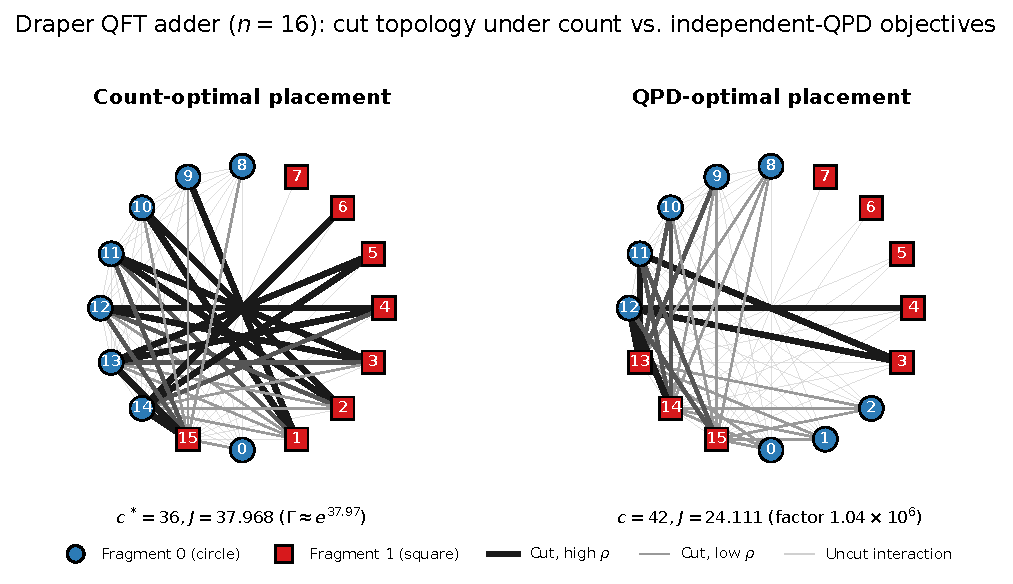
\includegraphics[width=0.92\textwidth]{figures/fig_draper_n16_topology.pdf}
  \caption{Draper QFT-adder interaction topology at $n=16$ under exact balanced bipartition. Left: count-optimal placement ($c^*=36$, $J\approx37.97$). Right: independent-QPD-optimal placement ($c=42$, $J\approx24.11$). Darker cut edges carry larger $\log\rho$; the QPD plan trades cut count for avoidance of high-overhead controlled phases.}
  \label{fig:draper-topology}
\end{figure*}

\begin{table}[t]
\centering
\caption{Identity-free heterogeneous-QPD companion corpus. All costs come from Qiskit's independent-QPD registry.}
\label{tab:heterogeneous}
\begin{tabular}{lr}
\toprule
\textbf{Metric} & \textbf{Value}\\
\midrule
Instances & 120 (5 families; $n\in\{12,14,16\}$)\\
Strict reversals & 16 (13.3\%)\\
Median / p90 factor & $5.30\times$ / $27.47\times$\\
Extra cuts, median / max & 1 / 3\\
Avoided iSWAP cuts & 28\\
Numerically closed & 120/120\\
\bottomrule
\end{tabular}
\end{table}

\begin{table}[t]
\centering
\caption{Algorithm-derived MQT~Bench audit. ``Max factor'' is descriptive over six fixed sizes per family, not a population estimate.}
\label{tab:e6-summary}
\begin{tabular}{lrrr}
\toprule
\textbf{Family} & \textbf{Eligible} & \textbf{Reversals} & \textbf{Max factor}\\
\midrule
Draper QFT adder & 6/6 & 4/6 & $1.04\times10^6$\\
HHL & 6/6 & 0/6 & $1$\\
Exact QPE & 6/6 & 2/6 & $4.03$\\
Inexact QPE & 6/6 & 0/6 & $1$\\
QFT & 6/6 & 0/6 & $1$\\
Entangled QFT & 6/6 & 0/6 & $1$\\
\bottomrule
\end{tabular}
\end{table}

\begin{table}[t]
\centering
\caption{Grouped nonzero-delta gate-class accounting for the Draper $n=16$ witness. The groups sum to $+6$ cuts and $J_{\rm QPD}^*-J_{\rm count}^*=-13.856805$; full per-angle accounting is in the reproducibility artifact.}
\label{tab:e6-draper}
\begin{tabular}{lrrr}
\toprule
\textbf{CP angle class} & \textbf{Count} & \textbf{QPD} & $\boldsymbol{\Delta c}$\\
\midrule
$-\pi/64$ through $-\pi/4$ & 5 & 13 & $+8$\\
$\pi/64$ through $\pi/16$ & 6 & 15 & $+9$\\
$\pi/4$ & 5 & 2 & $-3$\\
$\pi/2$ & 6 & 2 & $-4$\\
$\pi$ & 6 & 2 & $-4$\\
\midrule
Total & 28 & 34 & $+6$\\
\bottomrule
\end{tabular}
\end{table}

\subsection{Capacitated $K$-way heterogeneous scaling}
\label{sec:results-kway}

We evaluate the core formulation~\eqref{eq:kway} beyond bisection on a frozen heterogeneous-QPD benchmark of 144 runs (three fixed seeds per family--size--$K$ cell, $n\le60$, $K\le5$, 10-s SCIP limit). Table~\ref{tab:e9-kway} and Fig.~\ref{fig:e9-closure} summarize all runs, including open cases. SCIP reaches solver-tolerance closure on $101/144$ runs. The boundary is strongly graph- and seed-dependent: community matching and weighted repeat close all three seeds through $(K,n)=(3,60)$ and $(4,40)$, whereas random matching is the hard family---all three $K=2,n=60$ runs close, but every $K\geq3,n\geq40$ run remains open.

The factors quantify why closure alone is insufficient. Across the three random-matching $n=32,K=5$ runs, the median open factor is $10^{15.47}$; at $n=60,K=4$ it is $10^{44.84}$. The latter is deliberately prominent: it is an extreme resource-risk bound, not a near-optimality result. These values state that the corresponding incumbents carry no useful solver-tolerance multiplicative overhead guarantee at this deadline, and their explicit reporting prevents an unproven incumbent from being presented as an optimum. Thus this study establishes a practical baseline and a transparent computational boundary, not universal large-$K$ scalability. The exact-capacity comparison also expresses the fragment-width/overhead tradeoff directly: increasing $K$ reduces the maximum fragment size while generally forcing more independent-QPD boundaries (Fig.~\ref{fig:e9-pareto}).

We further confirm that cut count is a poor proxy for sampling overhead at the placement level using matched-objective heuristics that solve the same fixed independent gate-QPD, exact-capacity $K$-way problem: greedy swap, a count-weighted pairwise Kernighan--Lin (KL) adaptation, QPD-weighted KL, and KaHIP-QPD with exact-capacity repair~\cite{kernighanlin1970,kahip}. One canonical evaluator recomputes $J$, fragment sizes, and cut occurrences for every method, and also re-evaluates each reported SCIP incumbent after decoding it to a discrete partition. On the 101 solver-tolerance-closed records (Table~\ref{tab:e9-heuristic}), KL-QPD matches the SCIP objective on 68 records with median $\log_{10}R=0$ and p90 $2.94$, whereas count-weighted KL matches only 23 with median $\log_{10}R=1.56$; the two differ only in objective semantics within one heuristic family, isolating the effect of optimizing overhead rather than count. All 144 partitions from every matched method satisfy exact capacities. We also apply the same native independent-QPD model to 36 algorithm-derived MQT~Bench circuits: SCIP closes 15 within 10~s, KL-QPD matches all 15 solver-tolerance-closed objectives, and the six Draper-adder records form the largest structured positive subset. Three VQE candidates are retained as explicit ingestion failures because their native two-qubit operations lack a Qiskit QPD basis. Thus the heuristic finding is not solely a synthetic-graph artifact.

\begin{table}[t]
\centering
\tabfitscript
\caption{Capacitated $K$-way heterogeneous-QPD scaling, three fixed seeds per cell and a 10-s SCIP limit. ``Closed'' means solver-tolerance closure. Open records retain finite factors, including $10^{44.84}$ at random-matching $n=60,K=4$; this fixed matrix is not a workload-prevalence estimate.}
\label{tab:e9-kway}
\tabfit{%
\begin{tabular}{lccc}
\toprule
\textbf{Family} & \textbf{Closed} & \textbf{All-seed closure frontier} & \textbf{Boundary}\\
\midrule
Random matching & 24/48 & $K2,n60;K4,n20$ & $K\geq3,n\geq40$\\
Community matching & 37/48 & $K3,n60;K4,n40$ & $K5,n\geq32$\\
Weighted repeat & 40/48 & $K3,n60;K4,n40$ & $K\geq4,n=60$\\
\midrule
Total & 101/144 & $n=60,K=3$ & family/seed dependent\\
\bottomrule
\end{tabular}
}
\end{table}

\begin{table*}[tp]
\centering
\caption{Matched-objective baseline results. Regret statistics use 101 solver-tolerance-closed records only. KaHIP time includes an unbounded native call and is not budget matched ($\dagger$).}
\label{tab:e9-heuristic}
\tabfitstar{%
\begin{tabular}{lrrrrrr}
\toprule
\textbf{Method} & \textbf{Feasible} & \textbf{SCIP-obj. match / closed} & \textbf{Med. $\Delta J$} & \textbf{Med. $\log_{10}R$} & \textbf{p90 $\log_{10}R$} & \textbf{Med. time}\\
\midrule
Greedy swap & 144/144 & 23/101 & 3.33 & 1.45 & 10.52 & 0.100 s\\
Count-weighted KL & 144/144 & 23/101 & 3.59 & 1.56 & 5.01 & 0.100 s\\
KL-QPD & 144/144 & 68/101 & 0.00 & 0.00 & 2.94 & 0.100 s\\
KaHIP-QPD + repair & 144/144 & 51/101 & 0.00 & 0.00 & 1.47 & 5.89 s$^\dagger$\\
\bottomrule
\end{tabular}
}
\end{table*}

\begin{figure*}[tp]
  \centering
  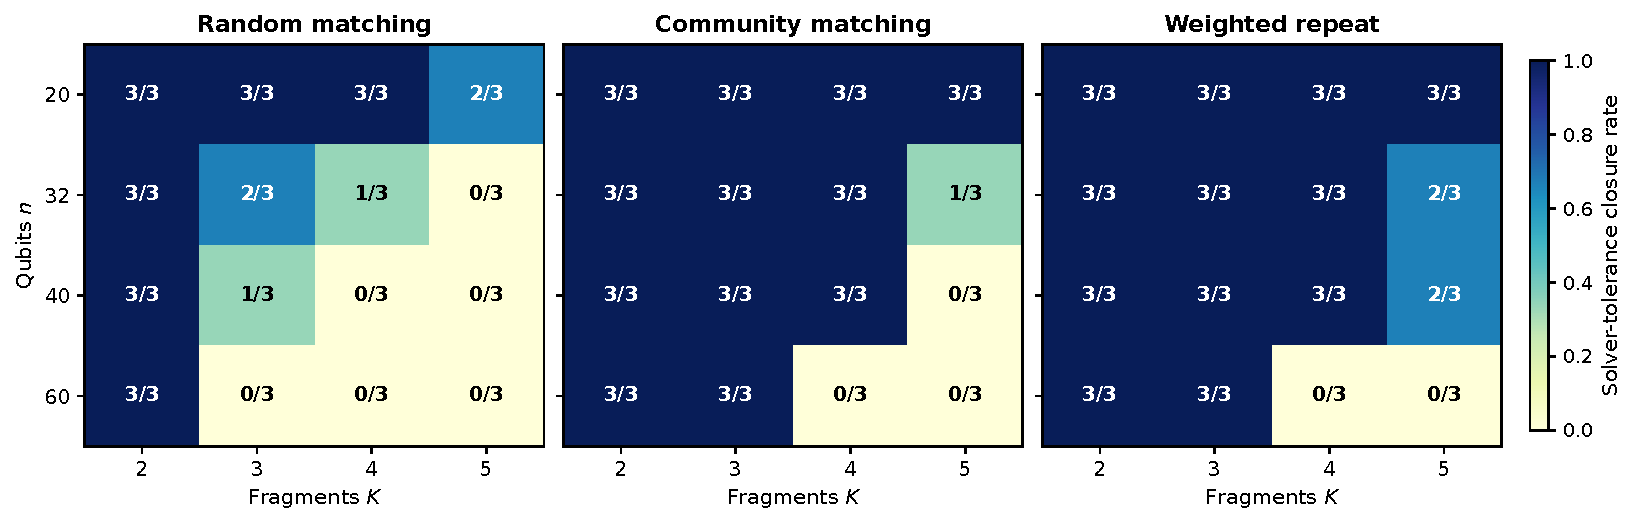
\includegraphics[width=0.72\textwidth]{fig_e9_closure_heatmap.pdf}
  \caption{Solver-tolerance closure counts under a 10-s SCIP limit. Each heatmap cell reports closed runs out of three fixed seeds. The boundary depends materially on graph family, $K$, and seed.}
  \label{fig:e9-closure}
\end{figure*}

\begin{figure}[t]
  \centering
  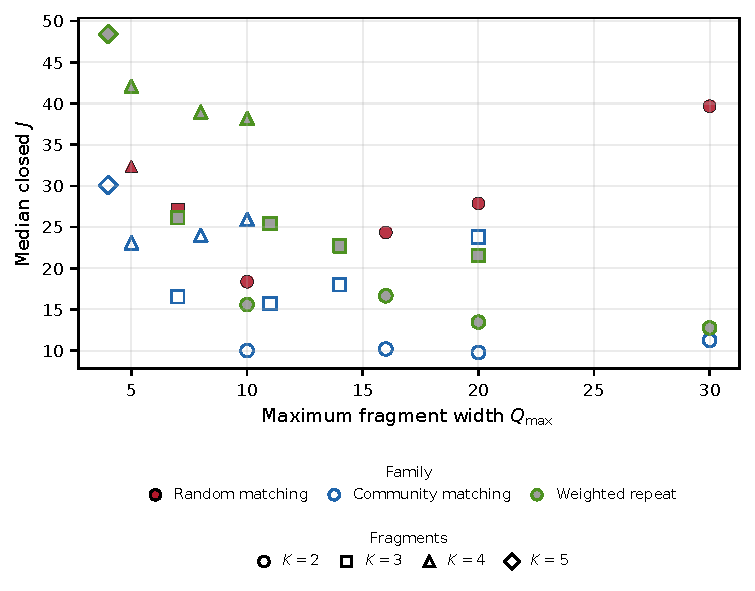
\includegraphics[width=\columnwidth]{fig_e9_width_overhead_pareto.pdf}
  \caption{Width--overhead tradeoff restricted to cells closed for all three seeds. Colors denote families, with distinct fill treatments (filled, open, gray-filled) so that families remain distinguishable in grayscale; markers denote $K$. Each point is the median solver-tolerance-closed log-objective $J$ for its cell.}
  \label{fig:e9-pareto}
\end{figure}

\subsection{Sensitivity to the quasiprobability resource model}
\label{sec:results-joint}

Independent QPD is a declared cut-cost model, not an assertion that stronger joint decompositions preserve placements. We therefore test whether the optimal placement can itself depend on the assumed resource model. Under a theorem-guarded library of pairwise-disjoint same-layer gate groups, a controlled six-qubit witness makes the independent optimum $1.90496\times$ worse when evaluated under a restricted parallel-joint semantics: a model-induced placement reversal exists. This is the resource-model analogue of the representation reversals of Sec.~\ref{sec:results-reversals}---there the interaction weights change because the gate-level representation changes; here they change because the assumed decomposition changes---and it shows that the placement decision is a function of the declared resource model as well as of the circuit.

We then test algorithm-derived native-QPD circuits under the same restricted pair library. The joint-aware MIP matches exhaustive enumeration on all 17 records with $n\le12$ and finds no strict independent-to-joint reversal in that subset, despite eligible saving opportunities. This is a scope stress test, not a claim that \CertiCut{} optimizes general joint QPD or that joint models cannot change algorithmic placements; general joint-QPD-aware partitioning, together with wire-cut and hybrid gate/wire models, remains future work~\cite{schmitt2025,ufrecht2024,brenner2025}. We emphasize that the framework as optimized targets the independent per-gate model exclusively, and we quantify rather than conceal the gap to a stronger model.

\subsection{Finite-shot scope}
\label{sec:results-shot}

A final study fixes an equal total ideal-Aer shot budget on three predeclared $n=12$ witnesses. The strong $719.66\times$ modeled reversal reduces RMSE for both observables, whereas a moderate $3.27\times$ reversal is mixed and a no-reversal control is identical under shared seeds. Hence independent-QPD overhead can be operationally informative but is not claimed as a universal finite-shot RMSE predictor. Full witness identities, signed-estimator behavior, and bootstrap intervals remain in the artifact. This study evaluates finite-shot behavior in an ideal-simulator implementation rather than modeling it.

% ===================================================================
% VI. RELATED WORK
% ===================================================================
\section{Related work}
\label{sec:related}

Peng \emph{et al.}~\cite{peng2020} introduced circuit cutting for evaluating circuits wider than the available quantum device, building on quasiprobability simulation~\cite{bravyi2016}. Mitarai and Fujii developed virtual-gate constructions and overhead bounds for nonlocal channel simulation~\cite{mitarai2021,mitarai2021overhead}. CutQC couples automatic partitioning with classical recombination~\cite{tang2021}, while Qiskit Addon Cutting implements gate-level QPD experiment generation and reconstruction~\cite{qiskitcutting}. Recent work studies multi-unitary, joint, and communication-assisted cutting~\cite{schmitt2025,piveteau2022,ufrecht2024,ufrecht2023,piveteau2024,piveteau2025sideinfo,brenner2025,lowe2023,li2024,shotqc2024,golden2023,gentinetta2024,carrera2024,harrowlowe2025}. Hardware-aware work optimizes mixed gate/wire cuts, heterogeneous device partitions, routing overhead, or hardware-noise constraints~\cite{mosaiqc2026,tw2s2026,pal2026noise}, and complementary distributed-QPU work develops multilevel temporal-hypergraph partitioning for teleportation and communication cost~\cite{burt2026}. \CertiCut{} instead fixes a logical interaction graph and independent \emph{gate}-QPD registry to obtain an exact placement formulation and explicit solver-tolerance resource-bound semantics; these objectives are complementary rather than direct regret comparators.

Qiskit Addon Cutting~0.10.0~\cite{qiskitcutting} supports SparsePauliOp-oriented workflows. \CertiCut{} is designed to feed that stack: the MIP returns a capacitated partition and an independent-QPD cut set whose sampling overhead is certified in the same multiplicative model that the addon uses to generate and recombine subexperiments. Table~\ref{tab:scope-comparison} positions the evaluated scope quantitatively where reported by the cited papers; heterogeneous cut models, capacity semantics, and bound types preclude a direct speed ranking. Nakamura \emph{et al.}~\cite{nakamura2025} study sampling bounds and scalable partitioning beyond bipartitions; ScaleQC, FitCut, QRCC, and Circuit Folding pursue scalable hybrid or distributed cutting workflows~\cite{scaleqc2022,fitcut2024,qrcc2025,circuitfolding2025}; and Fr{\"o}hler \emph{et al.}~\cite{frohler2026} provide a broad heuristic framework for combined gate cuts, wire cuts, and joint gate groups. Brandhofer \emph{et al.}~\cite{brandhofer2024} optimize richer circuit-knitting partitions that jointly select gate and wire cuts, ancilla insertions, and classical communication; Idan \emph{et al.}~\cite{idan2026} establish NP-completeness for general cut placement and use SMT for bounded-size fragments; and Nannicini \emph{et al.}~\cite{nannicini2022} formulate optimal qubit assignment and routing as integer programming. These works address broader cut mechanics, routing, or execution resources; \CertiCut{} instead holds the logical wire set and feasible partition space fixed while analyzing representation-sensitive interaction weights. Weighted graph partitioning, branch-and-bound bounds, fixed-capacity cardinality, metric inequalities, and partitioning orbitopes are established optimization machinery~\cite{deza1997,lawler1966,kaibel2008}; we do not claim them as new. Our contribution is the model specialization, the resource-interpretable bound semantics, and the representation-placement theory above. As Appendix~\ref{app:backend} shows, we make no claim that a specialized branch and bound dominates general-purpose optimization; on the evaluated corpus the opposite holds.

\begin{table}[t]
\centering
\caption{Scope comparison with related cut-placement work. ``--'' means the cited work does not report a directly matching quantity. Values are not speed comparisons.}
\label{tab:scope-comparison}
\footnotesize
\setlength{\tabcolsep}{2pt}
\begin{tabular}{p{0.20\columnwidth}p{0.46\columnwidth}p{0.25\columnwidth}}
\toprule
\textbf{Work} & \textbf{Cut model and reported scale} & \textbf{Optimization evidence}\\
\midrule
Nakamura \emph{et al.}~\cite{nakamura2025} & Multi-fragment gate/wire objective; benchmark circuits, no matched fixed-$K$ capacity matrix & Scalable partitioning heuristic/objective comparison\\
Brandhofer \emph{et al.}~\cite{brandhofer2024} & Gate and wire cuts; up to 40 qubits, 51 gates at 1 h & Optimal mixed-cut formulation\\
Fr{\"o}hler \emph{et al.}~\cite{frohler2026} & Gate, wire, joint gate groups; random circuits through 1000 qubits & Heuristic placements, 50 runs/instance\\
\CertiCut{} & Fixed independent gate-QPD, exact capacities; $n\le60$, $K\le5$, 144 runs & Global SCIP solver-tolerance $\UB/\LB$ factors\\
\bottomrule
\end{tabular}
\end{table}

% ===================================================================
% VII. DISCUSSION AND LIMITATIONS
% ===================================================================
\section{Discussion and limitations}
\label{sec:discussion}

The results establish circuit representation, and more generally the assumed quasiprobability resource model, as a relevant degree of freedom in resource-aware circuit cutting. The tie-safe metric~\eqref{eq:regret} is essential to that claim: the six QFT ``reversals'' that vanish under set-level comparison (Sec.~\ref{sec:results-qft}) show that a single-optimum analysis can report large spurious regret, so the perturbation bound (Proposition~\ref{prop:regret-bound}) and stability theorem (Theorem~\ref{thm:stability}) provide the quantitative conditions under which a placement decision is guaranteed to survive a representation change. Positive-scaling invariance (Corollary~\ref{cor:scaling}) explains the observed QAOA stability without any numerical search.

Several limitations bound these conclusions. The core formulation is restricted to gate-cut partitions under a fixed circuit representation, logical interaction graph, and independent per-gate QPD registry. Each optimization instance fixes one representation; the representation-regret study compares separate fixed-representation instances but does not jointly optimize over representation choice and partition placement. The formulation supports arbitrary declared $K$ and capacity bounds but does not optimize wire cuts, exact global routing, hardware noise, or an end-to-end physical execution objective. Joint QPD can reduce sampling overhead when compatible cut gates admit a collective decomposition, but its structural cost semantics lie outside the independent per-gate model optimized here; the restricted-joint study of Sec.~\ref{sec:results-joint} demonstrates model sensitivity rather than a general joint optimizer. The sparse $K$-way LP relaxation is weak, and the dense cardinality/metric extension of Appendix~\ref{app:poly} improves neither closure nor runtime at the reported scale. The benchmark matrices use three deterministic seeds per cell and remain fixed designs rather than workload-prevalence estimates; random-matching $K\geq3$ instances retain weak factors at 10~s, including an open factor of $10^{44.84}$. Finally, empirical optimization bounds are obtained from floating-point solvers: they are solver-tolerance quantities and, except for the interval tier of Appendix~\ref{app:verified}, have not been independently verified using directed rounding, rational reconstruction, or another rigorous lower-bound procedure. Reproducing the reported numbers requires the frozen protocol; changing the solver stack requires regenerating the evidence.

% ===================================================================
% VIII. CONCLUSION
% ===================================================================
\section{Conclusion}
\label{sec:conclusion}

We have shown that semantically equivalent quantum-circuit representations can alter the optimal placement of circuit cuts under a fixed independent-QPD model, and we have given the tools to certify when they do. A tie-safe set-level regret separates genuine representation-induced reversals from optimizer tie-breaking artifacts; a perturbation bound and a stability theorem quantify when a placement is guaranteed to survive a representation change; and positive-scaling invariance explains an entire family of stable cases analytically. Empirically, an exact QPE instance exhibits a placement-regret factor of $R=729$, six apparent QFT reversals collapse to $R=1$ under the tie-safe definition, and an exhaustively enumerated count-versus-QPD witness exceeds a factor of one million. For a fixed representation, capacitated $K$-way gate cutting under independent per-gate QPD reduces exactly to log-domain weighted graph partitioning, so any valid global bound pair $(\UB,\LB)$ yields the multiplicative resource bound $\Gamma_{\mathrm{inc}}/\Gamma^*\le\exp(\UB-\LB)$. A restricted joint-decomposition study shows that the optimal placement can depend on the assumed resource model as well as on the representation. \CertiCut{} packages this analysis, its exact formulation, and its frozen evidence as an auditable, resource-interpretable framework for independent-QPD circuit-cutting optimization, and it isolates representation as a degree of freedom that resource-aware cutting workflows should account for.

% ===================================================================
% BACK MATTER
% ===================================================================
\begin{acknowledgments}
The authors thank the maintainers of the open-source tools used in this work (Qiskit, Qiskit Addon Cutting, MQT~Bench, KaHIP, and SCIP) for enabling reproducible experimentation.
In accordance with APS policy, the authors disclose the use of generative AI assistants to assist in implementing and debugging experiment and analysis code; all code, results, and manuscript content were reviewed, verified, and validated by the authors, who take full responsibility for the work.
\end{acknowledgments}

% ---------------------------------------------------------------
% AUTHOR CONTRIBUTIONS (CRediT). VERIFY and edit to reflect the real
% division of labor before submission. Do NOT assign a role to an
% author who did not perform it. Placeholder below assigns all roles to
% the corresponding author and leaves H.B.'s roles to be confirmed.
% ---------------------------------------------------------------
\section*{Author contributions}
P.~T.~Hung: conceptualization, methodology, software, formal analysis, investigation, visualization, and writing---original draft. H.~Bui: supervision, and writing---review and editing. Both authors reviewed and approved the final manuscript and take responsibility for its content.

\section*{Data availability}
The data and software that support the findings of this study---including the reference implementation, the frozen raw records underlying every reported table and figure, the experiment scripts and solver configurations, and SHA-256 integrity manifests together with the pinned software versions, seeds, and solver tolerances needed to reproduce them---are provided to editors and referees at submission as a frozen review snapshot, and will be openly released in a versioned, DOI-bearing public repository upon acceptance~[DOI to be inserted].

% ===================================================================
% APPENDICES
% ===================================================================
\appendix

\section{Optimization backends and reference implementation}
\label{app:backend}

This appendix records the optimization backends behind the results of Sec.~\ref{sec:results}. The scientific claims of the paper do not depend on which backend supplies the valid bounds required by Theorem~\ref{thm:gap}; we retain a specialized reference search only as an independent algorithmic reference and, on the evaluated corpus, an off-the-shelf MIP solver outperforms it.

\subsection{Validation oracles and relaxations}

We use a compact MIP and brute-force enumeration as independent validation oracles. For one pair $(i,j)$, the convex hull of $x_{ij}=|z_i-z_j|$ is described by
\begin{equation}
\begin{aligned}
  x_{ij} &\geq z_i-z_j, & x_{ij} &\geq z_j-z_i,\\
  x_{ij} &\leq z_i+z_j, & x_{ij} &\leq 2-z_i-z_j.
\end{aligned}
  \label{eq:xor}
\end{equation}
The implementation uses an equivalent one-hot assignment model whose MIP retains only the two lower inequalities in~\eqref{eq:xor} and declares $x_{ij}$ binary; for positive-weight interacting pairs, minimization sets $x_{ij}$ to its exact XOR value. SciPy/HiGHS solves this MIP, while exhaustive enumeration through 16 qubits supplies a second oracle. Neither oracle contributes bounds to the anytime results. The basic reference LP (A0) uses one-hot assignment variables and cut variables only for interacting pairs, retains exact balance and the two lower XOR inequalities from~\eqref{eq:xor}, and relaxes all variables to $[0,1]$; because the weights are nonnegative, this is a valid but weak lower relaxation.

\subsection{Exact balanced $K\!=\!2$ reference problem}

The specialized reference implementation uses the $K=2$ exact-balanced special case. All legacy reference circuits have even $n$; the reference requires $n/2$ qubits per fragment and fixes $z_0=0$ to remove label symmetry:
\begin{equation}
  \min_{z \in \{0,1\}^n} \sum_{i<j} w_{ij}\,|z_i - z_j|
  \quad \text{s.t.} \quad \textstyle\sum_i z_i = n/2,\; z_0 = 0.
  \label{eq:balanced}
\end{equation}
Every feasible bisection cuts exactly $(n/2)^2$ pairs in the complete-pair representation, $\sum_{i<j}x_{ij}=n^2/4$, the special case of~\eqref{eq:kway-cardinality} used by the strengthened relaxation of Appendix~\ref{app:poly}.

\subsection{Reference branch and bound and its safe boundary}

The reference optimizer maintains open nodes in nondecreasing order of their LP bounds, expands the best-bound node, fathoms integral nodes after updating the incumbent whenever it improves $\UB$, and otherwise branches on the most fractional unfixed label. Child LPs reuse the root cut pool of Appendix~\ref{app:poly}; any child whose lower bound is at least $\UB$ is pruned. After all LP solves associated with an expansion complete, the algorithm reaches a \emph{safe boundary} and computes
\begin{equation}
  \LB = \min\!\left(\UB,\; \min_{N \in \mathcal{N}_{\mathrm{open}}} \LB_N\right),
  \label{eq:global-lb}
\end{equation}
with $\min_{N\in\emptyset}\LB_N=+\infty$, so that $\LB=\UB$ when the frontier is empty. The additive log-domain gap and multiplicative overhead factor are $\gap=\UB-\LB$ and $F=\exp(\gap)$.

\begin{proposition}[Reference safe-boundary validity, exact arithmetic]\label{prop:safe-boundary}
In exact arithmetic, every reference-search safe stopping boundary satisfies $\LB\leq\OPT\leq\UB$.
\end{proposition}
\begin{proof}
Feasibility of the incumbent gives $\OPT\leq\UB$. Every unexplored feasible solution belongs to a frontier subtree whose LP value lower-bounds all integral completions in that subtree. Equation~\eqref{eq:global-lb} therefore gives $\LB\leq\OPT$.
\end{proof}

Experimental deadlines are \emph{soft}: the reference optimizer stops only at a safe boundary, and we report the actual boundary time. Together with Theorem~\ref{thm:gap}, Proposition~\ref{prop:safe-boundary} supplies the exact-arithmetic premise for the anytime resource bound $\Gamma_{\mathrm{inc}}/\Gamma^*\le\exp(\UB-\LB)$; in practice every reported bound uses floating-point HiGHS or SCIP output and is a solver-tolerance quantity (Sec.~\ref{sec:num-semantics}). Figure~\ref{alg:certicut} states the full anytime search. Two greedy incumbents seed the search: H0 assigns vertices by descending weighted-degree greedy insertion with first-improving single swaps, while H2 adds a spectral (Fiedler) initialization and best-improving Kernighan--Lin swaps; neither establishes a lower bound.

\begin{figure}[t]
\centering
\fbox{\begin{minipage}{0.94\columnwidth}
\small
Algorithm: Anytime \CertiCut{} reference search\medskip\\
\textbf{Input:} QPD-weighted interaction graph $G$, capacity $q_{\max} = n/2$, soft deadline $T$.\smallskip\\
\textbf{Step 1.} Compute initial feasible partition and upper bound: $(P_{\mathrm{inc}}, \UB) \leftarrow \textsc{H2}(G)$.\smallskip\\
\textbf{Step 2.} Solve and strengthen root LP via separation: $(\LB_0, \mathcal{C}) \leftarrow \textsc{B2S\text{-}Root}(G)$. Freeze cut pool~$\mathcal{C}$.\smallskip\\
\textbf{Step 3.} Initialize search frontier $\mathcal{N}_{\mathrm{open}}$ with the root node.\smallskip\\
\textbf{Step 4.} While $\mathcal{N}_{\mathrm{open}} \neq \emptyset$ and elapsed time $< T$:
\begin{itemize}\setlength{\itemsep}{0pt}
  \item Select the open node $N^*$ of least lower bound $\LB_{N^*}$.
  \item If $N^*$ is integral, update the incumbent when it improves $\UB$, then fathom $N^*$.
  \item Otherwise, branch on the most fractional unfixed qubit; solve child LPs using $\mathcal{C}$; prune children with $\LB_N\geq\UB$.
\end{itemize}\smallskip
\textbf{Step 5.} At each safe boundary, compute the global lower bound~\eqref{eq:global-lb} and emit a bound report.\smallskip\\
\textbf{Output:} Best partition $P_{\mathrm{inc}}$ and bound report $(\LB, \UB, F = \exp(\UB - \LB))$.
\end{minipage}}
\caption{The \CertiCut{} reference anytime search for exact-balanced $K\!=\!2$ partitioning.}
\label{alg:certicut}
\end{figure}

\subsection{Mature MIP is the strongest evaluated backend}

Three SCIP variants differ in formulation strengthening: G0 is the sparse basic model (cut variables only for interacting edges and the two lower XOR inequalities, no cardinality); G1 augments G0 with complete-pair cut variables, the full XOR hull, and the cardinality identity $\sum x_{ij}=(n/2)^2$; and G2 further adds the full triangle/metric inequalities~\eqref{eq:tri1}--\eqref{eq:tri4}. Table~\ref{tab:e7-backends} reports all 200 frozen heterogeneous-QPD instances at each independent checkpoint. SCIP~G0 is the strongest practical backend among the evaluated methods, reaching solver-tolerance closure on 199/200 instances at 2~s and all 200 by 10~s; the specialized reference implementation closes 160/200, 184/200, and 199/200 at 2, 10, and 60~s. At 60~s the reference matches the G0 incumbent on 199/200 records, its single open case being a dense-shuffled $n=40$ instance with $F=6.1262$. Statically adding cardinality or full triangles to SCIP does not improve its end-to-end performance on this corpus. These results do not support a specialized-solver performance advantage; they show that the log-domain model-factor semantics can be instantiated by either the reference implementation or a mature MIP solver. All methods run single-threaded and, at each independent wall-clock checkpoint, emit common $\UB$, $\LB$, and $F=\exp(\UB-\LB)$ fields, which are solver-tolerance quantities.

\begin{table}[t]
\centering
\caption{Frozen heterogeneous-QPD backend comparison. Entries are counts with $F\leq1.01$; they equal solver-tolerance closures here. All factors and closures are solver-tolerance quantities.}
\label{tab:e7-backends}
\tabfit{%
\begin{tabular}{lrrrr}
\toprule
\textbf{Method} & \textbf{2 s} & \textbf{10 s} & \textbf{60 s} & \textbf{60 s UB match G0}\\
\midrule
Reference & 160/200 & 184/200 & 199/200 & 199/200\\
\textbf{SCIP G0} & \textbf{199/200} & \textbf{200/200} & \textbf{200/200} & reference\\
SCIP G1 & 111/200 & 186/200 & 196/200 & 198/200\\
SCIP G2 & 108/200 & 158/200 & 183/200 & 189/200\\
\bottomrule
\end{tabular}
}
\end{table}

\section{Polyhedral formulations and negative ablations}
\label{app:poly}

This appendix records the $K=2$ polyhedral strengthenings and the negative ablations that motivated the sparse production formulation of Sec.~\ref{sec:opt}. They are supporting context, not additional research claims.

\subsection{Balanced-cut cardinality and metric inequalities}

The B2S reference lifts A0 to the complete pair space, imposes the full XOR hull~\eqref{eq:xor}, and adds two families of valid constraints. \emph{Balanced-cut cardinality}: the identity $\sum_{i<j}x_{ij}=n^2/4$ from~\eqref{eq:balanced} fixes the total cut mass. \emph{Metric inequalities}: for each triple $(i,j,k)$, the cut polytope satisfies~\cite{deza1997}
\begin{align}
  x_{ij} - x_{ik} - x_{jk} &\leq 0, \label{eq:tri1}\\
  x_{ik} - x_{ij} - x_{jk} &\leq 0, \label{eq:tri2}\\
  x_{jk} - x_{ij} - x_{ik} &\leq 0, \label{eq:tri3}\\
  x_{ij} + x_{ik} + x_{jk} &\leq 2. \label{eq:tri4}
\end{align}
Inequalities~\eqref{eq:tri1}--\eqref{eq:tri3} are valid facets of the multiway-cut polytope for arbitrary $K$, whereas~\eqref{eq:tri4} is specific to the $K=2$ cut polytope and is imposed only in the $K=2$ formulations: for $K\ge3$, three qubits may occupy three distinct fragments, making $x_{ij}+x_{ik}+x_{jk}=3$ feasible. B2S solves the root LP, separates violated inequalities until none remain or the separation budget is exhausted, and reuses the resulting pool throughout the tree with no node-level separation.

\begin{proposition}[Objective-bound redundancy without cardinality]\label{prop:redundancy}
For nonnegative weights, adding~\eqref{eq:tri1}--\eqref{eq:tri4} to the complete-pair baseline CP0 does not change its optimal value. This is an objective statement, not a claim that the metric inequalities leave the CP0 polyhedron unchanged.
\end{proposition}
\begin{proof}
Take an optimal CP0 solution and retain its label vector $z$. Set $x_{ij}=|z_i-z_j|$ for every pair. This extension satisfies the pairwise XOR hull and all metric inequalities because absolute distance on the line is a metric and, for $z_i\in[0,1]$, $|z_i-z_j|+|z_i-z_k|+|z_j-z_k|\leq2$. For fixed $z$, these are the smallest feasible pair values; nonnegative weights therefore ensure that the objective does not increase, so the metric-augmented optimum is no larger than the CP0 optimum. The reverse inequality follows because constraints were added.
\end{proof}

\begin{proposition}[Relaxation validity]\label{prop:relax-valid}
The B2S LP optimum is a valid lower bound on the $K=2$ reference $\OPT$.
\end{proposition}
\begin{proof}
For binary labels, $x_{ij}=|z_i-z_j|$ satisfies~\eqref{eq:xor}. A balanced partition cuts $|F_0||F_1|=n^2/4$ complete-graph pairs, and each label triple satisfies~\eqref{eq:tri1}--\eqref{eq:tri4}. Hence every feasible integral bisection remains feasible in the relaxation, whose minimum cannot exceed $\OPT$.
\end{proof}

\begin{proposition}[Trivial sparse root relaxation]\label{prop:trivial-root}
For exact capacities $L_k=U_k=n_k$, the LP relaxation of the sparse edge-only formulation~\eqref{eq:kway} has objective zero.
\end{proposition}
\begin{proof}
Set $a_{ik}=n_k/n$ and $y_{ek}=n_k/n$ for every qubit $i$, edge $e$, and fragment $k$, then set $z_e=0$. Assignment and capacity equalities hold since $\sum_kn_k=n$. The upper AND inequalities hold at equality; the lower inequality holds because $n_k/n\geq2n_k/n-1$. Finally $z_e+\sum_ky_{ek}=1$. Thus this is LP feasible with zero nonnegative objective.
\end{proof}

\subsection{Negative ablations}

Motivated by Proposition~\ref{prop:trivial-root}, we tested an all-pair extension of~\eqref{eq:kway} that imposes~\eqref{eq:kway-cardinality} with auxiliary nonedge variables and complete-metric triangles. This is a negative ablation, not a proposed production formulation: for $K>2$, materializing all pair variables and triangle constraints expands the representation to $\Theta(n^2)$ pairs and $\Theta(n^3)$ triples, increasing LP construction, memory traffic, and reoptimization cost at every node, while adding only the multiway-cut-valid triangles~\eqref{eq:tri1}--\eqref{eq:tri3}. On a 36-record $n\in\{20,32\}$ ablation at 5~s, the base formulation closes 31 records, symmetry-only closes 29, and the cardinality or cardinality-plus-metric variants close 6 each. Production runs therefore use SCIP's sparse assignment/locality formulation with only the valid equal-capacity anchor.

Table~\ref{tab:root-decomposition} decomposes the root relaxation on 24 matched complete-pair instances: cardinality (C) and metric (T) inequalities become jointly effective only when combined (12/24 roots closed under CT versus 0/24 under CP0, C, or T alone), consistent with Proposition~\ref{prop:redundancy}. Table~\ref{tab:ablation} confirms B2S reference-search closure under a 100-node budget; it does not establish a production advantage over SCIP. Bound quality and incumbent quality are separate bottlenecks: on six predeclared random-matching cells ($n\in\{40,60\}$, $K\in\{3,4,5\}$, seed~0), the default and exact-cardinality root strengthenings give the solver-tolerance bound-factor trajectories of Fig.~\ref{fig:e12-dual-bound-profiles}, a bound-quality comparison only and not a universal tuning claim. Table~\ref{tab:n40} breaks down the largest legacy CNOT-only reference size ($n=40$) by graph family.

\begin{table}[htbp]
\centering
\caption{Root-relaxation decomposition on 24 circuit-derived instances. C and T separately match CP0 on every instance; CT denotes their combination. Gaps are in log-overhead units.}
\label{tab:root-decomposition}
\tabfit{%
\begin{tabular}{lrrrr}
\toprule
\textbf{Root formulation} & \textbf{Root-closed} & \textbf{Med. gap} & \textbf{p90 gap} & \textbf{Med. time}\\
\midrule
CP0 & 0/24 & 26.2935 & 52.4468 & 0.3211 s\\
CP0 + C & 0/24 & 26.2935 & 52.4468 & 0.3429 s\\
CP0 + T & 0/24 & 26.2935 & 52.4468 & 0.2832 s\\
CP0 + C + T & 12/24 & 0.2848 & 3.8761 & 2.3222 s\\
\bottomrule
\end{tabular}
}
\end{table}

\begin{table}[htbp]
\centering
\caption{Controlled ablation on 90 synthetic balanced instances under a 100-node budget. ``Closed'' means solver-tolerance gap at most $10^{-9}$. ``Node-lim.'' is a non-exclusive count.}
\label{tab:ablation}
\tabfit{%
\begin{tabular}{lcccc}
\toprule
\textbf{Configuration} & \textbf{Closed} & \textbf{Node-lim.} & \textbf{Med. nodes} & \textbf{Root / Tree (s)}\\
\midrule
A0 + H0 (basic)   & 41/90 & 56 & 100 & 0.000\,/\,2.059\\
A0 + H2            & 41/90 & 52 & 100 & 0.000\,/\,2.072\\
B2S-root + H0       & 90/90 &  0 &   1 & 0.260\,/\,0.060\\
B2S-root + H2       & 90/90 &  0 &   1 & 0.256\,/\,0.063\\
\bottomrule
\end{tabular}
}
\end{table}

\begin{table}[htbp]
\centering
\caption{Family-level performance breakdown at $n = 40$ for the legacy CNOT-only reference. Each family contains ten seeded instances.}
\label{tab:n40}
\tabfit{%
\begin{tabular}{lccc}
\toprule
\textbf{Family} & \textbf{Solver-tol. closed} & \textbf{Med. time (s)} & \textbf{p90 time (s)}\\
\midrule
Community        & 10/10 &  0.809 &  1.186\\
Nearest-neighbor & 10/10 &  1.646 &  1.764\\
QAOA ring        & 10/10 &  5.367 &  6.173\\
Noisy-community  &  9/10 &  2.419 & 18.188\\
Random           & 10/10 & 18.344 & 41.224\\
Dense            & 10/10 & 24.070 & 52.669\\
Weighted-random  &  8/10 & 37.215 & 60.067\\
\bottomrule
\end{tabular}
}
\end{table}

\begin{figure}[t]
  \centering
  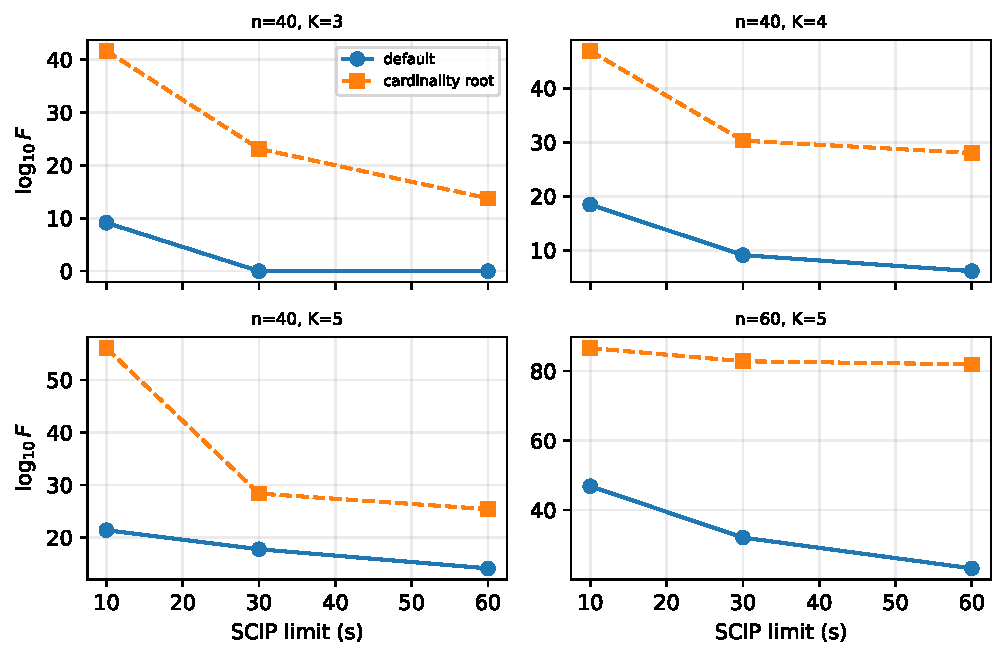
\includegraphics[width=\columnwidth]{fig_e12_dual_bound_profiles.pdf}
  \caption{Solver-tolerance bound-factor trajectories on representative predeclared random-matching cells. Lower values indicate tighter solver-tolerance bounds; each point is an independent bounded SCIP run.}
  \label{fig:e12-dual-bound-profiles}
\end{figure}

\section{Verified interval tier and reconstruction check}
\label{app:verified}

To ground the word ``certificate'' in a rigorously verified setting, a small CX-only tier is certified using exact interval arithmetic rather than SCIP bounds. It exhaustively enumerates 20 exact-input balanced-bipartition records with 80-decimal directed intervals for $\log 9$: nine have a uniquely separated optimum, and the remaining records certify the optimum objective in the presence of ties. Interval widths are $2\times10^{-79}$ to $3\times10^{-78}$, so these optima are numerical proofs up to verified outward rounding, not solver-tolerance estimates. This is the only tier for which we use \emph{certificate} in the strong sense; it is an enumerative interval oracle that verifies objective values independently but does not verify production SCIP lower bounds.

Independently, a shot-free statevector reconstruction check (Table~\ref{tab:operational}) confirms that predicted and Qiskit-derived overheads agree at machine precision, validating the cost accounting used throughout.

\begin{table}[htbp]
\centering
\caption{Statevector reconstruction check. Predicted and Qiskit-derived overheads agree; ``Abs. error'' compares reconstructed and uncut observables.}
\label{tab:operational}
\tabfit{%
\begin{tabular}{lcccc}
\toprule
\textbf{Circuit} & \textbf{Cuts} & \textbf{Pred. $\Gamma$} & \textbf{Exec. $\Gamma$} & \textbf{Abs. error}\\
\midrule
QAOA $n\!=\!6$, native $RZZ$ & 2 & 33.9706 & 33.9706 & $1.39\!\times\!10^{-17}$\\
VQE $n\!=\!6$, CX             & 1 & 9       & 9       & $5.55\!\times\!10^{-17}$\\
\bottomrule
\end{tabular}
}
\end{table}

Finally, we record the experiment-to-artifact map used by the reproducibility package (Table~\ref{tab:experiment-map}); the E-labels are artifact identifiers, not narrative units.

\begin{table}[htbp]
\centering
\caption{Experiment-to-artifact map. Primary narrative evidence is the count-versus-QPD, capacitated-scaling, and representation-regret studies; remaining rows are supporting context.}
\label{tab:experiment-map}
\begin{tabular}{llp{0.52\columnwidth}}
\toprule
\textbf{Role} & \textbf{Set} & \textbf{Question}\\
\midrule
Supp. & E1 & Legacy CNOT-only characterization of the reference implementation.\\
Supp. & E2/E3 & Dependence on CX-normalized versus native representation.\\
Supp. & E4 & Overlap with Qiskit's practical multi-fragment cutter.\\
Primary & E5/E6 & Tie-safe count-versus-QPD reversals.\\
Primary & E7 & Strongest $K=2$ anytime backend on heterogeneous-QPD instances.\\
Supp. & E8 & Finite-shot correspondence at equal budget.\\
Primary & E9 & Replicated $K\in\{2,3,4,5\}$ closure and bound factors through $n=60$.\\
Primary & E10 & $K$-way boundary on algorithm-derived native-QPD circuits.\\
Primary & Rep.-regret & Representation-induced placement reversal and stability.\\
Supp. & E12-D/E13/E15 & Root-bound profiles, restricted joint-QPD, interval enumeration.\\
\bottomrule
\end{tabular}
\end{table}

% ===================================================================
% REFERENCES
% ===================================================================
\bibliography{references}

\end{document}
